\documentclass{article}
\usepackage{graphicx}
\title{Implementation of the exponential function}
\author{P.L.~Bæk}
\date{}
\begin{document}
\maketitle
\begin{abstract}
We show some basic capabilities of the LateX system: math, figures,
references, sections...
\end{abstract}
\section{The Exponential Function}
The natural exponential function is defined as the function which is given as
\begin{equation}
	f(x) = e^x \;\;\;\; \textit{where} \;\;\; e=2.71828...
\end{equation}
This function is its own derivative:
\begin{equation}
	\frac{d}{dx}e^x=e^x\log_e e = e^x
\end{equation}
In a plot, the exponential function looks as shown on Figure 1.
\begin{figure}
	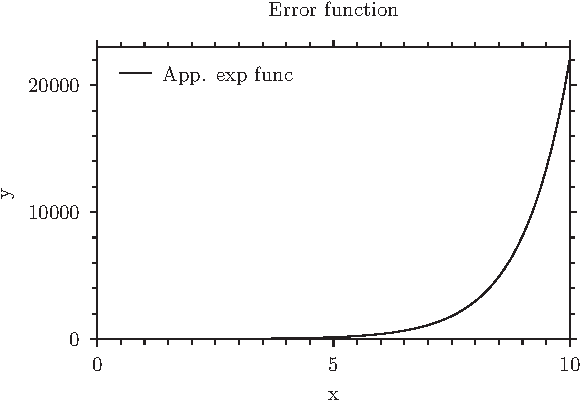
\includegraphics{fig-pyxplot-2.pdf}
\end{figure}


\section{Approximations}
As was shown from Figure 1, the exponential function is positive for all $x\in \mathcal{R}$. To describe the function at $x<0$ we see that we should converge towards 0 for $x\rightarrow -\infty$. A function that does exactly that is $1/-x$, which ensures a positive sign while the fraction ensures the convergence towards 0. \newline
When looking at the values of $x>0$ we see that the function behaves as a parabular function therefore making it tempting to approximate by $x^2$.
\newline
When $x$ is around origin, we can use a power expansion on the exponential funciton which can be shown to give
\begin{equation}
	e^x=\sum_n \frac{x^n}{n!}=1+x\left(1+\frac12 x\left(1+\frac13 x\left(...\right)\right)\right)
\end{equation}
Plotting the approximate exponential function on top of the real, we acquire figure 2
\begin{figure}
	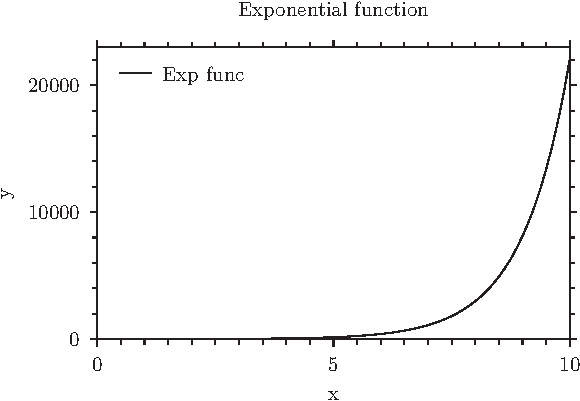
\includegraphics{fig-pyxplot.pdf}
\end{figure}
\end{document}
~
